\documentclass[sigconf, anonymous=false, screen=true]{acmart}

%% HotMobile 2027 submission — 8-page version with all 7 review patches applied.
%% Source: user's HotMobile draft + 7 patches (Challenges, prior-art gap,
%% Goals, n=7 fix, LongBench K=512, closed-loop framing, reproducibility).

\settopmatter{printacmref=false}
\renewcommand\footnotetextcopyrightpermission[1]{}
\pagestyle{plain}

\usepackage{booktabs}
\usepackage{tabularx}
\usepackage{multirow}
\usepackage{xcolor}
\usepackage{hyperref}
\usepackage{microtype}
\usepackage{graphicx}
\graphicspath{{figures/}}
\usepackage{algorithm}
\usepackage{algpseudocode}
\usepackage{enumitem}

%% --- Column-overflow control (added 2026-07-26) ---------------------------
%% TeX cannot break a text-mode "/" or an inline \mathrm{clip}(...) group, and
%% cannot hyphenate \texttt identifiers, so slash-ladders, long code names and
%% wide inline math were bleeding up to 118pt past the column edge.
%% \slb = breakable slash; \ub = breakable underscore; emergencystretch soaks
%% up the remaining small (<25pt) text overflows.
\newcommand{\slb}{/\allowbreak}
\newcommand{\ub}{\_\allowbreak}
\setlength{\emergencystretch}{2em}

\definecolor{kvgreen}{RGB}{40, 174, 96}
\definecolor{kvred}{RGB}{192, 57, 43}
\definecolor{kvgray}{RGB}{85, 85, 85}
\newcommand{\good}[1]{\textcolor{kvgreen}{\textbf{#1}}}
\newcommand{\bad}[1]{\textcolor{kvred}{\textbf{#1}}}
\newcommand{\nodata}{\textcolor{kvgray}{\textit{---}}}
\newcommand{\circled}[1]{\raisebox{.5pt}{\textcircled{\raisebox{-.9pt}{\footnotesize #1}}}}

\begin{document}

%% Short running title (added 2026-07-26): the full title overflowed the running
%% head and collided with the venue string on every odd page.
\title[$\mu$KV: Closed-Loop KV Cache Eviction for Mobile LLM Inference]{$\mu$KV: Closed-Loop KV Cache Eviction with a Cheap Per-Head Gate, Per-Prompt Adaptive Dispatcher, and Cache-as-Thermal-Actuator for Mobile LLM Inference}

\author{Md Romyull Islam}
\affiliation{%
  \institution{Kennesaw State University}
  \city{Marietta}
  \state{Georgia}
  \country{USA}
}
\email{romyullislam2012@gmail.com}

\begin{abstract}
On a phone the KV cache, not compute, limits sustained LLM decode: cache size sets per-step DRAM reads, reads set power, power sets temperature, and temperature sets the throttle. Prior eviction policies were evaluated on server GPUs with perplexity as the only metric, and prior thermal-aware mobile systems act on frequency alone with no cache signal. We present $\mu$KV, a sequence-level KV eviction system for mobile inference. $\mu$KV scores and selects inside the flash-attention prefill graph through a small side node, so scoring costs the same as vanilla prefill; it evicts at the sequence level and compacts the cache with a 290\,ms state round-trip; it sets its budget from expected output demand rather than prompt length; and a reduce-only watchdog lowers the clock in small steps before the kernel throttle would engage. On a OnePlus 15 under a cold-start protocol with canonical baseline configurations, $\mu$KV decodes WikiText at 4.8$\times$ vanilla throughput with 62\% less system energy, retaining a 22.5\,MiB cache against vanilla's 304\,MiB (a 13$\times$ reduction, all at the same self-limited 1.6\,GHz clock), and it does the work in 2.6$\times$ less time at 7\,\textdegree C lower skin temperature. The same measurements expose a realizability gap: per-head evictors such as SnapKV and Ada-KV cannot compact a sequence-level cache on a real inference engine, so their nominal budgets never materialize on the device. On needle-in-a-haystack retrieval $\mu$KV retrieves 7/7 at 4K on all three models with its bounded cache. We report costs as plainly as wins: on a WikiText slice verified disjoint from the prompt, $\mu$KV matches the full cache within 2\% perplexity on all three models, so what eviction costs is verbatim recall of the spans it drops, not language-modeling quality; and coupling cache size to temperature does not cap heat, so frequency remains the thermal lever.
\end{abstract}

\keywords{Mobile LLM inference, KV cache eviction, FlashAttention, thermal management, energy efficiency, Snapdragon, on-device AI}

\maketitle

\section{Introduction}
\label{sec:intro}

\paragraph{Motivation.} Phone LLM workloads differ from a server's: a single user, a 30--60\,s sustained generation, a thermal envelope that throttles long before any compute limit, and an OS that kills the process past a memory-headroom threshold. Quality is necessary but not sufficient; a policy that wins perplexity at the cost of skin temperature, peak resident-set, or battery drain fails deployment. The literature optimizes \emph{one} axis at a time (perplexity, DVFS, or compression alone), but the phone couples all of them: cache size sets DRAM read, read sets power, power sets temperature, temperature sets throttle, throttle sets throughput. A mobile KV-cache policy must be jointly evaluated on \emph{quality} (NIAH, LongBench, perplexity), \emph{throughput} (decode tps at realistic 16K context), and \emph{thermal} (peak DDR vs the kernel cliff, peak skin, watchdog activity), on real hardware. The literature has nothing that does all three on a phone.

\paragraph{Problem.} Small instruction-tuned LLMs (1--4B parameters, 4-bit quantized) now run interactively on flagship phones at 5--7 tokens/s on CPU. The remaining wall is not the matrix multiply; it is the KV cache. Once sustained generation passes a thousand tokens, four pressures bind at once:

\begin{itemize}
\item \textbf{Cache size.} A Phi-3-mini cache at 2K holds about 1.2\,GiB (f16 K+V). On a 12\,GB phone shared with foreground apps this triggers swap: 158\,MB of swap-out under the full cache, swap-in stalls near 280\,ms.
\item \textbf{DRAM bandwidth.} Decode reads the whole cache once per layer per token, roughly 750\,MB per attention pass for Phi-3 at 2K. On LPDDR5X (${\sim}50$\,GB/s) this dominates the step.
\item \textbf{Thermals.} The Qualcomm BCL~\cite{qualcommbcl} and the kernel cooling driver cut the big-core clock from 1632 to 883\,MHz once DDR passes about 65\,\textdegree C, often within 90\,s of sustained decode.
\item \textbf{Energy.} A full-cache 2048-token decode draws about 38.7\,mAh; on a 5000\,mAh battery that is about 130 generations before any other app load.
\end{itemize}

\paragraph{Five design challenges.} A phone-viable evictor must resolve five tensions no single prior mechanism handles together. (i) Any per-head signal from post-softmax attention is locked out of FlashAttention, the kernel that makes mobile decode fast. (ii) q8\_0 K quantization only pays above roughly a 1\,GB cache, since below that the dequantize cost exceeds the bandwidth saving (\S\ref{sec:eval-cross}). (iii) Aggressive eviction runs \emph{hotter} at peak, not cooler, because the freed bandwidth converts to clock and power; the envelope is set by peak temperature, not total energy. (iv) A fixed $K$ wastes headroom on short prompts while a fraction-of-prompt $K$ blows the DRAM budget on long ones. (v) At a tight budget the same ramp tunes either for chat throughput (small $K$, recent-heavy) or document-QA quality (large $K$, anchor-heavy), so the split should be chosen per request from a cheap prefill signal. $\mu$KV addresses these with in-graph scoring on the flash-attention path, a precision ablation, steady-state cache reduction, an honest fail-mode disclosure, and an adaptive-anchor dispatcher that sets $\alpha_a\in[0.05,0.95]$ per prompt from the distant-sharpness fraction of prefill attention (\S\ref{sec:design}).

These pressures are coupled: the system informally minimizes $\alpha_1 \text{Wall} + \alpha_2 \text{Energy} + \alpha_3 \text{Jitter}$ subject to a perplexity budget, a peak-temperature ceiling, and a total-I/O ceiling. One intervention, bounding the cache by a per-head confidence-aware budget, pushes on all four pressures at once.

The policies that could supply that bound were designed elsewhere: H2O~\cite{zhang2023h2o}, TOVA~\cite{oren2024tova}, SnapKV~\cite{li2024snapkv}, StreamingLLM~\cite{xiao2024streamingllm}, and the per-head allocator Ada-KV~\cite{feng2025adakv}, all built for server GPUs and measured by perplexity alone. On our hardware canonical H2O is 32\% \emph{slower} than the full cache at decode, because reading attention scores each step forces the FlashAttention-off path.

We test two questions on a real phone. First, whether attention-driven eviction plus a thermal control loop can win on throughput, energy, peak RSS, and thermal margin: yes, and with the mass-based $\alpha_a$ dispatcher on retrieval too, where the earlier count-based configuration failed buried-fact retrieval but the completed 336-cell phone NIAH sweep retrieves 7/7 at 4K on every model at a fixed 1024-cell cache (Table~\ref{tab:phone-niah-prelim}); the residual quality cost is confined to verbatim recall of evicted spans, not to language modeling, which stays at full-cache perplexity (\S\ref{sec:eval}). Second, whether cache size can serve as a thermal actuator, unlike prior thermal-aware mobile systems (zTT~\cite{kim2021ztt}, FUSE~\cite{liu2022fuse}, ZeroDVFS, Qualcomm BCL~\cite{qualcommbcl}) that act on CPU/GPU frequency only: no, a thermally coupled cache budget does not cap peak temperature (\S\ref{sec:eval-tdak}), so frequency remains the thermal lever and the cache an efficiency lever.

\paragraph{Contributions.} Per-head adaptive budget allocation is Ada-KV's idea~\cite{feng2025adakv}; we credit it and do not reprove its bound. We claim four contributions, ordered by what carries the measured win:

\begin{enumerate}[label=(\roman*),leftmargin=*,itemsep=2pt]
\item \textbf{A cheap closed-form per-head gate plus a per-prompt adaptive dispatcher} (\S\ref{sec:design}). Each head's budget $K_h$ comes from its max-of-softmax $m_h$ through one ramp, which costs $O(H)$ per layer against Ada-KV's $O(HN\log HN)$ global top-$B$ and needs no variable-length kernel. A mass-based dispatcher, $\alpha_a$ = the fraction of attention mass lying outside the recent window (clipped to $[0.05, 0.95]$), then auto-selects the anchor:recent split from the same tensor anchor selection uses (one column-mean reduction, no extra forward pass). These two layers carry the throughput-energy win.

\item \textbf{Keeping a score-reading evictor on the flash-attention fast path} (\S\ref{sec:design}). Reading post-softmax attention normally forces the slow FA-off path; $\mu$KV computes its selection scores inside the FA-on prefill graph via a small \texttt{kq\_evict} side node emitted only on the last prefill chunk, so prefill costs the same as vanilla. A 290\,ms state round-trip then compacts the cache in place (CPU; on the GPU the transfer is prohibitive and the cache stays sparse, \S\ref{sec:gpu-results}), and prefill, selection, and decode all run FA-on. To our knowledge no prior attention-driven evictor runs entirely on the fast path on a phone.

\item \textbf{A reduce-only thermal watchdog that makes the kernel throttle unreachable} (\S\ref{sec:eval-thermal}). A userspace daemon reads skin, battery, DDR, and CPU sensors and lowers the clock cap one step at a time as calibrated thresholds approach, never raising it; it runs only under $\mu$KV and stays dormant on a cold phone, keeping the deeper mitigations (the 883\,MHz cliff, battery-current events) unreachable. We also report a negative result: coupling the cache budget to temperature does not cap heat (\S\ref{sec:eval-tdak}), which is why clock and cache remain separate actuators.

\item \textbf{First end-to-end mobile measurement} of attention-driven KV eviction. Nine policies on a OnePlus 15 under a cold-start protocol with canonical baselines, reporting temperature, per-phase system energy, retained cache, per-step KV state, and CPU clock traces, none of which prior KV-cache work reports on a phone. The measurements expose a realizability gap: per-head evictors (SnapKV, Ada-KV) cannot compact a sequence-level cache, so their nominal budgets never materialize, while $\mu$KV's sequence-level selection compacts to 22.5\,MiB against vanilla's 304\,MiB, a 13$\times$ reduction.
\end{enumerate}

$\mu$KV is the eviction-and-thermal half of a larger closed-loop controller for sustained mobile LLM inference: model-internal signals (per-head attention concentration here, per-step output entropy in a companion paper) drive cache state, hardware-internal signals (temperature, eventually flash write count) drive frequency and I/O. Disclosing where the eviction half breaks (\S\ref{sec:limitations}) motivates the per-request selection the closed loop will provide.

\paragraph{Non-goals.} We do not claim a new theoretical bound on eviction loss (Ada-KV~\cite{feng2025adakv} owns that), a new attention-score signal (KVzip's reconstruction-attention~\cite{kim2025kvzip} is orthogonal), zero retrieval loss at the throughput corner (C5 is real and we report it), a new mobile DVFS algorithm (we use one-way pinning and a multi-sensor watchdog as engineering baselines), or novelty for the state API itself. The contribution is the composition: attention-driven eviction + multi-sensor thermal control + cache-as-thermal-actuator, in one decode loop, end-to-end on a phone.

\section{Background and Related Work}
\label{sec:bg}

Autoregressive decode reads all cached keys and values each step, so per-step bandwidth grows with the cache; on mobile LPDDR5X this dominates beyond a few hundred tokens.

\textbf{Eviction policies} cut the cache to a budget $K$. H2O~\cite{zhang2023h2o} and TOVA~\cite{oren2024tova} keep heavy hitters or recent high-attention positions and must read attention scores every step. SnapKV~\cite{li2024snapkv} freezes a top-$K$ keep set at end of prefill. StreamingLLM~\cite{xiao2024streamingllm} keeps a few sink tokens plus a sliding window and needs no scores. Ada-KV~\cite{feng2025adakv} is the closest prior art for the per-head idea: it proves a tight $L_1$ eviction-loss bound, allocates a non-uniform per-head budget from a global top-$B$ over concatenated post-softmax attention, adds an $\alpha{=}0.2$ safeguard blending toward uniform $B/H$ so no head starves, and relies on FlashAttention-2's variable-length kernel~\cite{dao2023flashattention2} to keep heterogeneous head budgets fast on GPU. That kernel is absent on our mobile CPU stack, one reason we trade the global top-$B$ for a closed-form ramp needing one reduction per head. The same group extended this line with CriticalKV~\cite{feng2025criticalkv} and DefensiveKV~\cite{feng2025defensivekv}. AhaKV~\cite{gu2025ahakv} corrects the per-token \emph{score} under a uniform budget, orthogonal to a per-head \emph{budget} and compatible with ours. KIVI~\cite{liu2024kivi} compresses by 2-bit quantization rather than eviction. KVzip~\cite{kim2025kvzip} takes a different angle: a \emph{query-agnostic} score from prompting the LLM to reconstruct the prefilled context and recording per-pair max cross-attention, evicting pairs that contribute little; it reports near-lossless quality at 30\% budget on SCBench and RULER, and a head-level variant replacing DuoAttention's hours of head-score optimization with one minute of forward passes. KVzip is orthogonal on two axes: its reconstruction scoring costs roughly $2\times$ prefill (fine offline on servers, costly on-device, whereas our ramp adds zero forward passes), and its evaluation is GPU-only and quality-only, reporting no temperature, watt, or peak-RSS on a phone and still facing the FA-on/FA-off split. Our contribution is the on-mobile measurement, not a new importance signal; its reconstruction score could drop into our per-head gate as future work. None of these reports any thermal, power, or memory measurement on a mobile device.

\textbf{The architectural conflict} shaping $\mu$KV: FlashAttention~\cite{dao2022flashattention, dao2023flashattention2} fuses softmax into the kernel and never writes the attention tensor to DRAM, which makes it fast. A policy that reads attention scores cannot use the fused kernel, so score-reading evictors are locked to the slow path, which is why H2O loses throughput.

\textbf{Mobile and edge inference systems.} PowerInfer-2~\cite{song2024powerinfer2} and LLM in a Flash~\cite{alizadeh2023llm} optimize weight access, orthogonal to cache management. MLC-LLM~\cite{mlcllm} compiles models for mobile GPUs but uses the unmodified KV cache. ExecuTorch (Meta) targets the on-device PyTorch runtime but leaves cache policy to the model author. MediaPipe LLM Inference (Google) and Apple's CoreML pipeline both use fixed-budget sliding-window caches. MNN-LLM and llama.cpp~\cite{llamacpp} expose the cache directly but ship no eviction policy. PerCache~\cite{liu2025percache} is the closest mobile-RAG counterpart: a predictive hierarchical cache combining a semantic QA bank with reusable QKV tensors, populated during idle time by asking an on-device LLM to predict future queries, reporting up to 34\% latency reduction on commodity phones. It is adjacent but disjoint from $\mu$KV: PerCache operates at the application level, shortcutting entire inference passes by matching queries against precomputed query-answer pairs and retrieved-chunk KV, and does not touch the per-step DRAM read pattern of the decode loop, whereas $\mu$KV operates inside the decode loop, bounding the cells attended per step. The two compose: PerCache decides \emph{whether} to run the loop, $\mu$KV \emph{how cheaply} when PerCache misses. PerCache reports no temperature, watt, or thermal-cliff data. None of these systems couples the cache axis to the thermal axis on a phone.

\textbf{Weight-side compression is orthogonal and complementary.} Per-token decode traffic is $S_\mathrm{weights}+S_\mathrm{KV}$: weight quantization (GPTQ, AWQ, K-quants in \texttt{llama.cpp}) and weight-sharing (MoE, weight tying) shrink the first term, KV eviction the second; they attack \emph{different} tensors and compose. Which dominates depends on context length: on a $\sim$4\,B Q4\_K\_M model the weights are $\sim$2.3\,GB and \emph{static}, while the KV cache \emph{grows} from ${\sim}0.2$\,GB at $K{=}512$ to ${\sim}3.6$\,GB at full 8K context on Phi-3, so in the long-context decode $\mu$KV targets, the KV term rivals or overtakes the weight term, exactly when eviction pays. Native 1-bit/ternary training pushes the weight term far down: PrismML's Bonsai-8B stores an 8.2\,B model in 1.15\,GB (${\sim}16\times$ smaller than FP16) with ${\sim}8\times$ faster decode and ${\sim}4$--$5\times$ better energy on edge hardware, from reduced weight-memory traffic~\cite{prismml2026bonsai}. This complements rather than competes: PrismML collapses $S_\mathrm{weights}$, $\mu$KV collapses $S_\mathrm{KV}$, and at long context a $16\times$-smaller-weight model \emph{still} pays full KV traffic, so $\mu$KV remains necessary on top; together they minimize per-token DRAM movement (and DDR heat) across the context-length range. $\mu$KV composes with any weight quantization, 4-bit or 1-bit.

\textbf{Energy-aware mobile and server inference.} zTT~\cite{kim2021ztt}, FUSE~\cite{liu2022fuse}, and ZeroDVFS act on CPU/GPU \emph{frequency} from temperature or workload phase but have no KV signal. Power-aware LLM serving systems (Sponge, Sheared, Toaster) target server-side batching, not the on-device thermal envelope. Carbon-aware schedulers (Carbon Containers, Treehouse) target the macroscale energy mix, not per-decode-step thermal control. RAPL-based governors apply on x86 servers but cannot read mobile DDR or skin sensors. Conversely, no published KV-cache work has a thermal signal. $\mu$KV is the first system to read attention-internal state \emph{and} hardware temperature sensors in one decode loop on commercial flagship phone hardware.

\textbf{Industrial on-device LLM efforts.} Apple Intelligence (iOS 18) runs a 3B model on the A18 NPU with adapter quantization and CoreML; standard sliding-window KV, closed source. Samsung Galaxy AI runs Gemini Nano plus on-device Llama-family models on the NPU; standard KV. Google Gemini Nano (Pixel 8+) exposes a $\sim$3B model through AICore; standard KV. Qualcomm AI Hub and the Snapdragon LLM SDK ship Hexagon-NPU references; standard KV. None publishes a KV-cache eviction policy with measured thermal, watt, or memory data on a mobile device. $\mu$KV occupies the gap: an open, attention-driven evictor with multi-sensor thermal control, evaluated end-to-end with full multi-axis numbers.

\paragraph{Where each prior policy breaks on a phone.} H2O reads attention each step, locked to FA-off: $-32\,\%$ decode throughput vs the full cache (Table~\ref{tab:master-wikitext}). SnapKV freezes a top-$K$ at end of prefill but allocates it uniformly per head, over-allocating sharp heads and starving broad ones. TOVA keeps per-head top-$K$ from the last query but with a uniform budget and stays FA-off. StreamingLLM keeps a sink plus a sliding window, always evicting the middle of the context, where buried-fact retrieval lives (\S\ref{sec:limitations}). Ada-KV's per-head allocator needs FA-2's variable-length kernel~\cite{dao2023flashattention2}, absent on the mobile CPU stack, and pays $-39\,\%$ decode throughput (Table~\ref{tab:master-wikitext}). KIVI~\cite{liu2024kivi} compresses with 2-bit quantization rather than evicting, orthogonal. \textbf{None reports a temperature, watt, peak resident-set, or swap byte on a phone.}

\paragraph{Why other policies do not save memory or energy on a phone.} \textit{Active KV cache} savings at $K{=}512$ are similar across evicting policies (all bound resident cells to $\le K{\cdot}H{\cdot}L$). But \emph{peak resident-set} (what matters for the OS killer and foreground-app headroom) tracks total process memory, not just the cache. Three asymmetries appear in our measurements (Table~\ref{tab:master-wikitext}, peak\_rss\_kb): (i) FA-off policies allocate a per-decode attention-scratch tensor of size $O(B {\cdot} H {\cdot} N {\cdot} K)$ that FA-on policies never materialize, an extra $\sim$120\,MB in H2O/TOVA/AdaKV on Phi-3 at $K{=}512$. (ii) Score-reading policies retain a full attention-score history buffer; $\mu$KV needs only the per-head $m_h$ scalar from prefill. (iii) Compaction drops the prefill scoring workspace before decode, freeing $\sim$80\,MB. Net: $\mu$KV's peak RSS is 9.3--13\,\% below the full cache, while H2O/TOVA/AdaKV match or exceed full-cache RSS despite a smaller \emph{active} cache.

\emph{Energy} savings work differently: they happen only when the policy stays FA-on. We measure $+45$--$95\,\%$ energy on H2O, TOVA, StreamingLLM, and Ada-KV (Table~\ref{tab:master-wikitext}) because their score-readback forces FA-off, multiplying decode wall time by $1.7$--$2.1\times$, which dominates the energy integral. $\mu$KV keeps scoring inside the FA-on graph and runs FA-on for thousands of decode tokens, so it is the only evictor delivering a measured energy win against the full cache.

\paragraph{Offloading is out of scope here.} Spilling evicted cells to flash instead of dropping them is a distinct design point that trades DRAM pressure for UFS endurance, bandwidth, and per-token latency. At the budgets $\mu$KV targets the working set already fits in DRAM (about 192\,MB at $K{=}512$ on Phi-3), so there is nothing to offload; offloading matters only in the unbounded-context regime and is treated in the companion whole-system paper alongside the flash write-count controller.

\section{$\mu$KV Design}
\label{sec:design}

$\mu$KV is a small set of cooperating mechanisms behind one decode loop (Figure~\ref{fig:architecture}). An \emph{inner loop} uses the prefill attention tensor $\bar A_{l,h,p}$ to set cache content: the per-head gate sizes a per-head budget from $\max_p \bar A$; anchor selection picks anchor positions from cross-head $\mathrm{mean}_{l,h} \bar A$; the dispatcher splits anchor:recent from the same column-mean as a per-prompt $\alpha_a$; eviction runs at the sequence level and compacts the cache, keeping decode FA-on; the cache stores K in q8\_0 to halve K-side bytes. An \emph{outer loop} reads skin, battery, DDR, and CPU sensors and caps CPU frequency in small steps before the kernel throttle engages. Figure~\ref{fig:mechanism} shows where the scores come from inside the attention computation.

\begin{figure*}[tp]
\centering
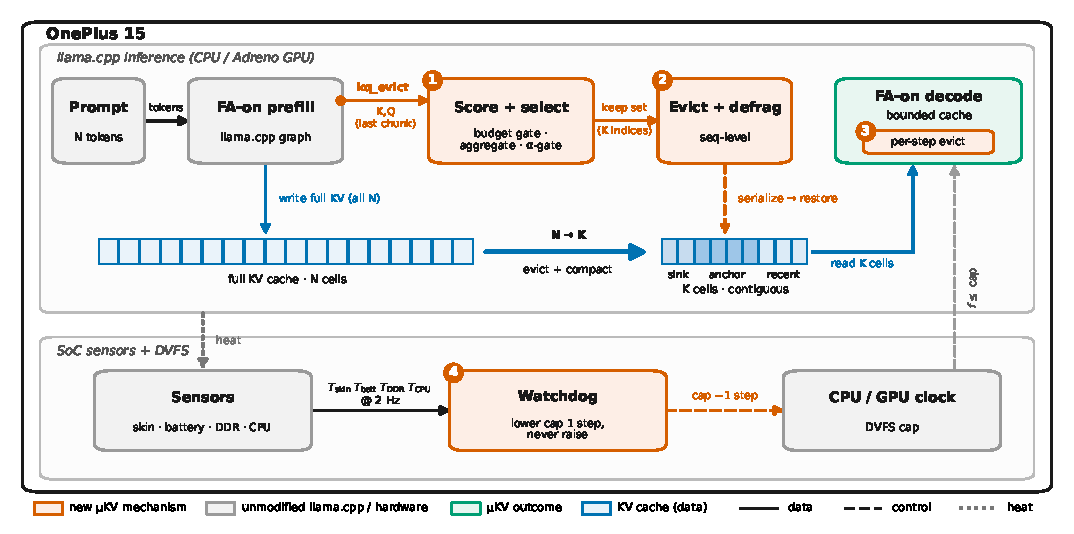
\includegraphics[width=0.94\textwidth]{figures/fig_architecture_v4.pdf}
\caption{$\mu$KV in the decode path. Orange marks new components: \circled{1} select, \circled{2} evict and compact, \circled{3} bounded FA-on decode, \circled{4} clock watchdog.}
\label{fig:architecture}
\end{figure*}

\begin{figure}[tb]
\centering
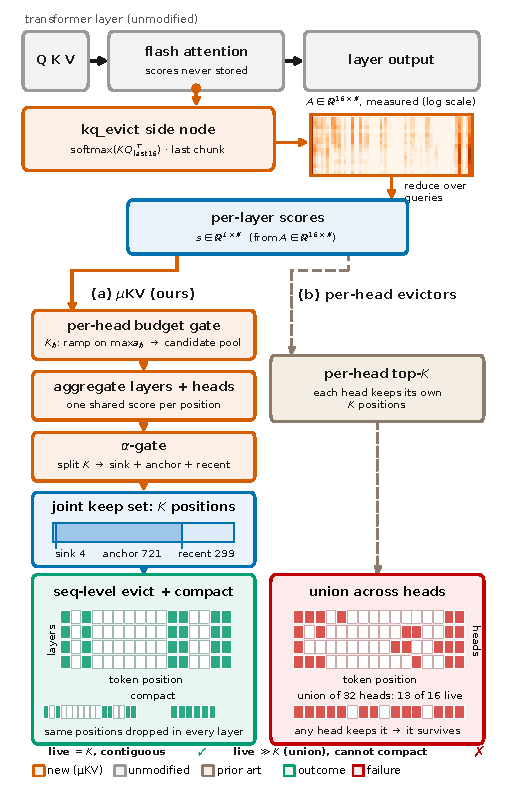
\includegraphics[width=0.94\columnwidth]{figures/fig_mechanism.pdf}
\caption{How $\mu$KV taps the attention computation and why sequence-level selection compacts while per-head selection cannot.}
\label{fig:mechanism}
\end{figure}


\textbf{K\_ceil-Ladder (prompt-aware K nominal).} Before prefill begins, a wrapper-layer ladder maps prompt length $N$ to the initial $K_\mathrm{nom}$:
\begin{equation}
\label{eq:kceil}
K_\mathrm{nom}(N) = \begin{cases}
N        & N \le 256 \\
512      & 256 < N \le 512 \\
1024     & 512 < N \le 1024 \\
K_\mathrm{MAX} & N > 1024
\end{cases}
\end{equation}
The ladder eliminates wasted budget on short prompts (a 50-token chat does not need a 1024-cell cache) and clamps long prompts to a deployable maximum. The selected $K_\mathrm{nom}$ flows into the per-head budget and anchor split. Cost: a single \texttt{strlen} plus a 4-way comparison, effectively free.

\paragraph{Why prompt length under-determines $K$, and how we choose it instead.} Eq.~\eqref{eq:kceil} rests on a false premise: that input length $N$ predicts the budget a request needs. It does not. Quality is governed by the \emph{effective attended span} (past positions with non-negligible attention mass at each decode step), which decouples from $N$ both ways. \emph{(i) Short prompt, long output.} A 20-token instruction (``write a 2000-word report'') emits thousands of tokens whose coherence depends on the \emph{growing generation}, so the span grows \emph{during} decode, independent of $N$; reasoning and long-form workloads make this acute, and micro-budgets ($<$128) \emph{backfire} into repetition loops generating \emph{more} tokens~\cite{cai2025rkv}. A prompt-length ladder gives such a request a tiny $K$, exactly wrong. \emph{(ii) Long prompt, short answer.} Retrieval/QA needs only a slice of a long prompt (attention concentrates on a few heavy hitters~\cite{zhang2023h2o}, and the query can be read from a prompt-end window before generation~\cite{li2024snapkv}), so $N$ \emph{over}-states the need; yet a fixed \emph{fraction} of $N$ can still evict a needle at intermediate depth~\cite{feng2025adakv}. Effective context is task-dependent, not length-dependent~\cite{hsieh2024ruler}, so task-aware budgeting~\cite{zhou2024dynamickv} beats length-keyed budgeting.

\emph{The stakes are physical, not just quality.} Across our 372-cell on-device dataset, $K$ is the master knob trading quality for \emph{both} speed and heat: a larger resident cache lowers decode throughput (memory\,$\leftrightarrow$\,tps, Pearson $r{=}{-}0.77$, the bandwidth-bound roofline) and raises DDR temperature (memory\,$\leftrightarrow$\,DDR, $r{=}{+}0.80$), and higher temperature in turn throttles throughput (tps\,$\leftrightarrow$\,DDR, $r{=}{-}0.71$). Over-provisioning $K$ wastes throughput and thermal margin, under-provisioning loses recall, so sizing $K$ sets the phone's sustainable operating point.

\emph{Demand-aware admission, then decode-time adaptation.} We keep $K$ as the actuator but re-found how it is chosen. At admission we size $K$ from the request's \emph{demand} rather than its input length:
\begin{equation}
\label{eq:kdemand}
\begin{aligned}
K_\mathrm{dem} &= \max\big(\,\underbrace{r(N)}_{\text{retrieval floor}},\ \underbrace{g(\hat L_\mathrm{out}, \text{task})}_{\text{generation floor}}\big),\\[2pt]
K_\mathrm{init} &= \mathrm{clip}\big(K_\mathrm{dem},\; K_\mathrm{min},\; \min(K_\mathrm{MAX},\, K_\mathrm{tier}(T_\mathrm{DDR}))\big),
\end{aligned}
\end{equation}
where $r(N)\!\le\!N$ covers the relevant prompt span (usually far below $N$); $g(\cdot)$ scales with the \emph{expected output length} $\hat L_\mathrm{out}$, often user-declared (``2000-word report'' $\Rightarrow \hat L_\mathrm{out}\!\approx\!2600$) or estimable from task class (chat $\sim$100, summary $\sim$200, report/reasoning $\sim$2000\,tokens); $K_\mathrm{min}\!\approx\!128$ is a hard floor against the micro-budget backfire; and $K_\mathrm{tier}(T_\mathrm{DDR})$ is the thermal admission cap. The \emph{generation} term is what Eq.~\eqref{eq:kceil} omits: the short-prompt/long-output request the ladder starves now receives budget matched to what it will \emph{generate}. During decode $K$ adapts on two signals: it \emph{grows} as $\hat L_\mathrm{out}$ is revised upward for open-ended tasks, and \emph{tightens} when the model is confident (low next-token entropy, the per-step gate of \S\ref{sec:discuss}), while the thermal ratchet supplies the downward emergency term, giving $K_t = \min\!\big(K_\mathrm{init}\!\uparrow_\text{gen},\, K_\mathrm{tier}(T_t)\big)$: demand raises $K$, heat lowers it. The load-bearing claim, that break-even $K$ tracks \emph{output} length not $N$, holds in a controlled retention test (Fig.~\ref{fig:kadaptive}). A fact is placed in a 36-token instruction, followed by a controlled span of $F$ tokens standing in for generation, then probed. The minimum $K$ that still retrieves it (the \emph{break-even $K$}) scales with output length ($256, 512, 1024, 2048, 4096$ as output grows $78\to2484$ tokens) and is essentially independent of the 36-token prompt. A prompt-length budget (the ladder's $K{=}36$) retrieves $0/5$, whereas a demand-aware $K$ from the expected output ($K\!=\!2{\times}(\text{prompt}{+}\hat L_\mathrm{out})$) retrieves $5/5$. An on-device sweep with real generation is underway to confirm the same surface with per-cell energy and thermals.

\begin{figure}[tb]
\centering
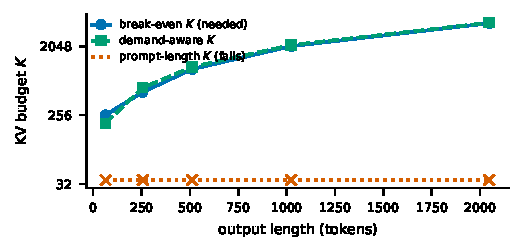
\includegraphics[width=\columnwidth]{figures/fig_kadaptive.pdf}
\caption{Break-even budget $K$ scales with output length, not with the fixed 36-token prompt (controlled retention test, Llama-3.2-1B).}
\label{fig:kadaptive}
\end{figure}


Eviction is position-based, so filler is a faithful stand-in for generated tokens.


\textbf{per-head budget.} At end of prefill, for each head $h$ we read the last query's post-softmax attention $A_h$ and take its peak $m_h = \max_p A_h^p$. A sharp head (large $m_h$) needs few cells, a broad head more. We map $m_h$ through a closed-form ramp
\[
\begin{gathered}
\mu(x) = 1.3 - 0.6\cdot\mathrm{clip}\!\left(\tfrac{x-0.4}{0.4},0,1\right)\in[0.7,1.3],\\[2pt]
K_h = \mathrm{round}(K_{\text{nom}}\,\mu(m_h)),
\end{gathered}
\]
keeping the top $K_h$ positions per head, union over heads clipped to $K_{\text{nom}}$. This is $O(H)$ per layer against Ada-KV's $O(Hn\log Hn)$ global top-$B$ and needs no variable-length kernel. The clamp $[0.7,1.3]$ plays Ada-KV's $\alpha$-safeguard role: no head starves or runs away. The breakpoints 0.4 and 0.8 come from the measured $m_h$ distribution on Phi-3, where heads with $m_h>0.8$ are about 22\% of heads but 51\% of attention mass. The ramp is a cheap mobile approximation, not Ada-KV's optimal budget.

\textbf{adaptive-anchor dispatcher ($\alpha_a$).} The per-head gate candidate pool $\bigcup_h S_h$ must split into ``anchor'' (distant) and ``recent'' fractions. Rather than a hand-tuned constant, we compute a per-prompt $\alpha_a$ from the same prefill attention tensor the per-head gate used. Letting $\bar{\bar A}[p]$ be the column-mean over $(l, h)$, define $\mathrm{distant\_mass} = \sum_{p < N - R_\mathrm{min}} \bar{\bar A}[p]$ and $\mathrm{total\_mass} = \sum_p \bar{\bar A}[p]$. Then
\[
\boxed{\;\alpha_a = \mathrm{clip}\!\left(\frac{\mathrm{distant\_mass}}{\mathrm{total\_mass}},\, 0.05,\, 0.95\right)\;}
\]
sets $n_\mathrm{anchor} = \mathrm{round}(\alpha_a \cdot (K_\mathrm{nom} - n_\mathrm{sink}))$ and $n_\mathrm{recent} = K_\mathrm{nom} - n_\mathrm{sink} - n_\mathrm{anchor}$. The cost is one column-mean reduction, the same reduction anchor selection already needs, so the dispatcher adds zero forward passes. Empirically (\S\ref{sec:eval-cross}, the mass-$\alpha_a$ ablation) $\alpha_a$ varies per prompt (0.62--0.95), auto-discovering the throughput corner on chat prompts and the quality corner on retrieval prompts without a deploy-time hyperparameter.

\textbf{selective anchoring.} The per-head union can retain hundreds of prompt cells and starve the recent window. We re-rank the union by mean cross-head attention and keep only the top $n_\mathrm{anchor}$ (from the dispatcher) as anchors, plus 4 sink tokens~\cite{xiao2024streamingllm}, leaving $n_\mathrm{recent}$ for the recent window. Without this cap, Phi-3 perplexity spiked to 158 in early runs.

\textbf{cache precision.} K is quantized to q8\_0, V kept at f16, a lighter profile than KIVI's 2-bit scheme~\cite{liu2024kivi} and free of training. This halves the K-side read and drops DDR temperature by about 3\,\textdegree C on Phi-3. On small models the dequantize cost can exceed the bandwidth saving, so it pays only above roughly 1\,GB cache (\S\ref{sec:eval-cross}).

\textbf{fast-path scoring and compaction.} The gate and dispatcher need post-softmax attention, which historically forced the slow FA-off path during prefill. $\mu$KV instead computes the scores inside the FA-on prefill graph through a small \texttt{kq\_evict} side node emitted only on the last prefill chunk (earlier chunks' scores are overwritten anyway), so selection is bit-identical and prefill costs the same as vanilla. A 290\,ms state serialize-and-restore pass then compacts the survivors into a contiguous cache, over which decode runs FA-on. An earlier variant ran prefill FA-off and swapped the compacted cache into an FA-on context; it selects the same cells but pays 10--15\% more prefill time, kept in the tables as $\mu$KV (state-swap). During decode a tiered re-eviction fires only when the active cache exceeds $1.25\times(n_{\text{anchor}}+B_R)$, amortizing eviction across many steps.

\textbf{watchdog.} A separate process samples DDR, CPU big-core, skin, battery temperature, and battery current at 2\,Hz, computes a per-sensor threat as the clamped warn-to-crit fraction, and takes the maximum. It lowers the big-core frequency cap one step at a time along direct temperature ladders anchored at the \emph{measured} deep-throttle trigger (battery 47.0\slb48.0\slb48.5\slb49.0\slb49.5\,\textdegree C and skin 50.0\slb51.0\slb51.5\slb52.0\slb52.5\,\textdegree C map to 1497\slb1382\slb1267\slb1132\slb1017\,MHz; DDR is a backstop only above 71\,\textdegree C, as it runs 66--69\,\textdegree C normally here), stepping down as thresholds approach and never rising above base, so it can only reduce. The thresholds are calibrated from the trigger we measured, not chosen in theory: on this SoC the vendor deep-throttle fires the instant battery reaches 50\,\textdegree C (Sec.~\ref{sec:eval-thermal}), and the ladder glides the clock below the vendor clamp through the 47--49\,\textdegree C run-up, with a 1017\,MHz floor above the 883\,MHz cliff. On a cold phone it stays dormant; its role is to replace the vendor's single deep drop to 883\,MHz with an early glide that, on a sustained workload, holds the battery below 50\,\textdegree C (Fig.~\ref{fig:bonsai-thermal}). The watchdog acts on one actuator: \emph{CPU frequency}.

\paragraph{Cost model.} Per decode step the wall time is bandwidth-bound: it scales with bytes read per step, set by the resident cache size and DDR bandwidth, the latter falling as DDR heats (the LPDDR5X refresh interval doubles near 85\,\textdegree C). Shrinking $K$ cuts bytes per step and so cuts both time and energy, but does not cap peak temperature: under sustained load frequency is the only lever that does (\S\ref{sec:eval-tdak}), which is why the watchdog acts on the clock and eviction on efficiency.
\paragraph{Three reductions of the same attention tensor.} The per-head gate, dispatcher, and anchor selection each take a \emph{different} reduction axis through the same captured tensor $\bar A_{l,h,p}$; none duplicates another:
\begin{itemize}[leftmargin=*, itemsep=2pt]
\item \textbf{the per-head gate (per-head row-max)} $\to$ per-head budget $K_h$: $m_h = \max_p \bar A_{l,h,p}$, then $K_h = \mathrm{round}(K_\text{nom}\cdot\mu(m_h))$.
\item \textbf{the dispatcher (cross-head column-mean partition)} $\to$ per-prompt anchor:recent split $\alpha_a$: $\bar{\bar A}[p] = \frac{1}{n_\text{layers}\,n_\text{heads}}\sum_{l,h} \bar A_{l,h,p}$, then $\alpha_a = \mathrm{distant\_mass}/\mathrm{total\_mass}$.
\item \textbf{anchor selection (column-mean top-K)} $\to$ which positions survive: $\mathrm{Anchor} = \mathrm{TopK}_{n_\text{anchor}}(\bar{\bar A})$.
\end{itemize}
The kept set is then $K = n_\text{sink} + n_\text{anchor} + n_\text{recent}$ with $n_\text{anchor} = \alpha_a(K-n_\text{sink})$ and the remainder a sliding recent window, so a reported budget of $K{=}1024$ means 4 sinks plus, e.g., 721 anchors and 299 recent, not 1024 anchors. Crucially this is \emph{one shared set across all heads}, which is what lets $\mu$KV compact on a sequence-level engine where per-head evictors cannot.
All three share the same $\bar A$ already captured for FA-off prefill, so no extra forward pass is needed.

\section{Evaluation}
\label{sec:eval}

\textbf{Setup.} OnePlus 15, Snapdragon 8 Elite Gen 5, 12\,GB UMA, CPU-only, 4 threads. Models: Phi-3-mini-128k, Llama-3.2-1B, gemma-2-2b-it, all Q4\_K\_M, run in a \texttt{llama.cpp} extension~\cite{llamacpp} we call \texttt{eviction\ub bench}. Each cell starts from a verified cool baseline (DDR/CPU $<$\,40\,\textdegree C; skin/PMIC/battery $<$\,36\,\textdegree C); USB charging is held OFF continuously by a per-cell keeper that re-disables every 30\,s (Android battery service otherwise re-enables charging mid-run). Per-cell sensor capture at 5\,Hz, with USB rail $V{\cdot}I$ integration for true system energy (\texttt{usb\_current\_ua}, \texttt{usb\_voltage\_uv}). $\mu$KV runs with mass-based $\alpha_a$ and the multi-sensor watchdog; baselines run as published.

\textbf{Two benchmarks at the same 16K context.}
\emph{(1) Sustained decode} (Table~\ref{tab:master-wikitext}). A $\sim$7K-token prompt (7.5K Phi-3 / 6.4K Llama-1B / 6.4K Gemma-2B) followed by 2K-token greedy generation with \texttt{-{}-ignore\allowbreak-eos}, in a 16{,}384-token allocated context (hence ``16K'' = KV-cache allocation, not prompt length). One run per (policy, model) cell. Measures the systems axes: throughput (decode tps), peak DDR/CPU/skin/PMIC/battery temperature, USB-rail energy, peak RSS, plus PPL on the decoded text. This is the workload that exposes thermal-cliff behavior because it sustains pressure for $\sim$10--50 minutes per cell.
\emph{(2) RULER-style NIAH retrieval} (Table~\ref{tab:phone-niah-prelim}). A buried-fact prompt: $\sim$5K--16K tokens of filler with the needle ``mango sorbet at Bi-Rite Creamery is the best thing to do in San Francisco'' inserted at one of 7 depths ($\{0, 17, 33, 50, 67, 83, 100\}\,\%$ of context), followed by ``Q: What's the best thing to do in SF?''. One run per (policy, model, context, depth). \emph{Hit} = generated text contains ``mango sorbet'' or ``bi-rite'' (case-insensitive). Measures the quality axis: can the policy retrieve a buried fact regardless of where it sits in the prompt? Total: 8 policies $\times$ 3 models $\times$ 14 depths (7 at 4K + 7 at 8K) $= 336$ cells, \textbf{all complete}: every model swept at both 4K and 8K.

\emph{Why both?} 16K-decode catches policies that fail thermal sustainability (slow or hot under long generation); NIAH catches policies that achieve speed by dropping information (StreamingLLM-style sliding window, which sweeps 16K-decode but fails NIAH because the needle gets evicted). Only a policy that wins BOTH benchmarks is deployable.



\begin{table*}[tp]
\caption{WikiText decode (9.7K prompt $+$ 4K decode, CPU-only, natural DVFS, cold start; nominal $K{=}1024$). Top block: Llama-3.2-1B Q4\_K\_M, all nine policies; bottom block: the same workload on PrismML's 1-bit Bonsai-8B. PPL$_\text{gen}$: self-generation perplexity. PPL$_\text{rec}$: teacher-forced perplexity on an eval slice that \emph{overlaps} the prompt, so it scores verbatim recall of retained text, not prediction; on a disjoint slice all policies match the full cache (see text). ActKV: retained live KV cells ($\mu$KV decode-mean in parentheses); Energy: total system power. Per-head policies do not compact on a sequence-level engine, so their ActKV stays high (see text).}
\label{tab:master-wikitext}
\centering\scriptsize
\setlength{\tabcolsep}{3pt}
\begin{tabular}{l l r r r r r r r r r r r}
\toprule
\textbf{Model} & \textbf{Policy} & \textbf{PPL$_\text{gen}$} & \textbf{PPL$_\text{rec}$} & \textbf{tps} & \textbf{Prefill (s)} & \textbf{Wall (s)} & \textbf{ActKV} & \textbf{$\alpha_a$} & \textbf{RSS (MB)} & \textbf{DDR (\textdegree C)} & \textbf{CPU (\textdegree C)} & \textbf{Energy (mWh)} \\
\midrule
\multirow{8}{*}{Llama-3.2-1B}
 & vanilla & 1.09 & 1.06 & 5.0 & 229 & 1055 & 9737 & --- & 2102 & 59.8 & 65.8 & 1033 \\
 & \textbf{$\mu$KV-mass-full} & 1.32 & 8.23 & \good{24.2} & \good{226} & \good{406} & 721 (1980) & 0.71 & 2154 & 54.4 & 63.5 & \good{391} \\
 & $\mu$KV (state-swap) & 1.11 & 8.03 & \good{22.7} & \good{250} & \good{438} & 733 (1984) & 0.72 & 2235 & 58.3 & 68.1 & \good{546} \\
 & SnapKV & 1.08 & 1.67 & 6.8 & 287 & 902 & 5929 & --- & 2236 & 56.3 & 63.1 & 818 \\
 & AdaKV & 1.09 & 2.63 & 6.7 & 252 & 875 & 3484 & --- & 2236 & 57.1 & 63.5 & 1002 \\
 & StrLLM & 1.22 & 8.57 & 6.6 & 250 & 877 & 777 & --- & 2236 & 56.7 & 63.5 & 1052 \\
 & H2O & 1.09 & 7.79 & 5.8 & 292 & 1006 & 6110 & --- & 2312 & 54.8 & 60.7 & 1094 \\
 & TOVA & 1.11 & 4.53 & 6.0 & 253 & 947 & 4091 & --- & 2235 & 54.4 & 60.7 & 1069 \\
\cmidrule(l){2-13}
\multirow{7}{*}{Bonsai-8B}
 & \textbf{$\mu$KV-mass-full} & 1.69 & 7.36 & \good{4.5} & 1073 & \good{2012} & 789 (1993) & 0.70 & 4517 & \good{62.5} & 79.5 & \good{2312} \\
 & vanilla & 1.10 & 1.12 & 1.0 & 1058 & 5137 & 10074 & --- & 4393 & \bad{72.2} & 79.8 & 5758 \\
 & SnapKV & 1.22 & 1.12 & 1.1 & 1103 & 4713 & 10015 & --- & 4475 & 67.9 & 81.4 & 5476 \\
 & AdaKV & 1.07 & 2.05 & 1.6 & 1191 & 3718 & 6514 & --- & 4580 & 65.2 & 76.0 & 3971 \\
 & StrLLM & 1.37 & 9.20 & 1.6 & 1161 & 3777 & 858 & --- & 4580 & 63.7 & 76.4 & 4012 \\
 & H2O & 1.12 & 7.89 & 1.5 & 1214 & 3900 & 9587 & --- & 4748 & 63.3 & 76.8 & 4136 \\
 & TOVA & 1.46 & 7.95 & 1.6 & 1149 & 3841 & 7116 & --- & 4580 & 67.2 & 87.6 & 4581 \\
%% Bonsai sweep complete (7 policies): mukv_faon + vanilla/snapkv/adakv/strllm/h2o/tova
\bottomrule
\end{tabular}
\end{table*}


\begin{figure}[tb]
\centering
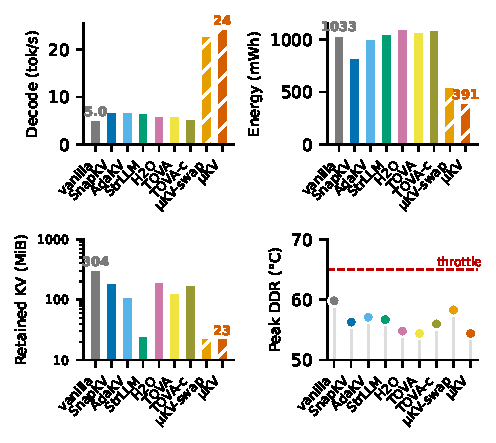
\includegraphics[width=\columnwidth]{figures/fig_main_results.pdf}
\caption{Per-policy results on WikiText (Llama-3.2-1B, cold start).}
\label{fig:main-results}
\end{figure}

\begin{figure}[tb]
\centering
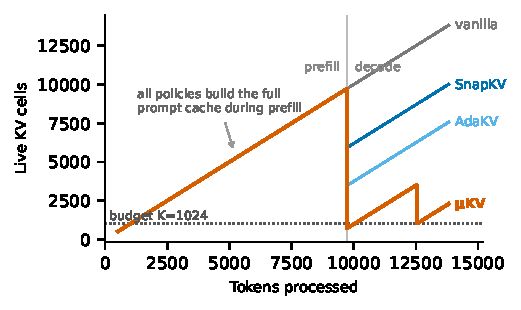
\includegraphics[width=\columnwidth]{figures/fig_cache_trajectory.pdf}
\caption{Live KV cells during prefill and decode.}
\label{fig:cache-trajectory}
\end{figure}


\paragraph{Measurement protocol.}\label{sec:revised-protocol}
All cells run on one build (aarch64, armv8.7-a, with the i8mm and repack kernels the Snapdragon 8 Elite supports) so throughput is comparable across policies. We let the vendor DVFS and thermal engine govern every cell, from a genuinely cold start (CPU and DDR below 37\,\textdegree C, shell below 34\,\textdegree C). We impose no artificial frequency cap; the vendor thermal engine governs the clock, and 1632\,MHz is not a hardware ceiling (the prime cores' OPP table reaches 4.6\,GHz). The prime cores do take their 2438\,MHz boost OPP during the cold, compute-bound prefill, but under the sustained bandwidth-bound decode the vendor engine clamps \texttt{scaling\ub max} to ${\sim}1632$\,MHz (and further to ${\sim}1498$\,MHz once the skin passes 41\,\textdegree C, which we observe live); the perf cores settle at ${\sim}1997$\,MHz. This clamp is set by temperature, not by us, and is identical for all nine policies, so the clock is not a confound and the throughput differences come from cache size and kernel path, not frequency. Charging stays disabled for the whole run so the state of charge is constant, and energy integrates total system power (USB rail plus battery discharge) split at the prefill/decode boundary. The retained-KV footprint is measured by \texttt{llama\ub state\ub seq\ub get\ub size}, which serializes live cells only; position-range counters over-state it. Every baseline runs its own paper's configuration with none of $\mu$KV's mechanisms: SnapKV uses the per-head FasterDecoding defaults (window 64, avgpool-5, top-$(K{-}64)$ from the prefix, no sinks); Ada-KV uses the Ada-SnapKV defaults (window 32, maxpool-7, $\alpha{=}0.2$ safeguard, no sinks); H2O keeps its 50/50 heavy-hitter and recent split with no sinks; StreamingLLM keeps its 4 attention sinks plus recent window; TOVA is realized in its paper-preferred per-layer form (Oren et al.\ average attention across a layer's heads) scoring from the last query, with a recent window that restores the recency TOVA holds emergently in streaming decode but loses when applied as a one-shot prefill selection, and we use this single per-layer TOVA in every benchmark (the strict no-recency form is a generation-mode variant that breaks only because the chunked-prefill last query is not the autoregressive token, a measurement artifact rather than a quality result, so we do not report it). The watchdog runs on $\mu$KV only and stays dormant from cold. $\mu$KV-mass-full combines FA-on prefill (in-graph scoring on the last chunk) with a 290\,ms post-eviction defrag, so it gets vanilla-class prefill and fast FA-on decode at once.

Two caveats. First, the PPL$_\text{rec}$ column measures recall, not quality, which is why we renamed it. Its evaluation text overlaps the prompt, so a policy that keeps the prompt can copy the answer. Vanilla's 1.06 is recall, not quality: holding the full context, it recognizes the passage and reproduces it. $\mu$KV's 8.23 is what a Llama-class model scores when it must actually predict. The column therefore ranks policies by how much prompt they retained, which is the thing under test.

We re-ran the measurement with the confound removed, on a WikiText slice verified disjoint from the prompt (0 of 159 sliding 200-character probes appear in it). On that slice $\mu$KV matches the full cache on every healthy configuration, after evicting about 92\% of the prompt cache:

\begin{center}\small
\begin{tabular}{l c r r r}
\toprule
\textbf{Model} & \textbf{runs on} & \textbf{vanilla} & \textbf{$\mu$KV} & \textbf{ratio} \\
\midrule
Llama-3.2-1B Q8\ub 0    & GPU & 8.198 & 8.023 & 0.98 \\
Phi-3-mini-128k Q4\ub K\ub M & GPU & 3.983 & 3.938 & 0.99 \\
Bonsai-8B Q1\ub 0 (1-bit) & CPU & 6.717 & 6.736 & 1.00 \\
\bottomrule
\end{tabular}
\end{center}

\noindent So eviction does not cost language-modeling quality. What it costs is verbatim recall of the spans it drops, which is exactly what the overlapping-slice number was measuring and what NIAH probes directly. Self-generation PPL is about 1.1 for every policy, and on NIAH (\S\ref{sec:eval}) $\mu$KV keeps the needle. We keep the recall column for continuity with prior work, which reports perplexity in this overlapping form, but we treat the disjoint slice and NIAH accuracy as the quality result. These runs are on a Jetson Orin NX, because scoring a disjoint slice needs a second full context alongside the prompt. The first two are GPU-resident (1252 and 2229\,MiB of weights on CUDA); the 1-bit Bonsai weights stay in the CPU repack buffer, since these cells predate our CUDA Q1\ub 0 port, so its row is CPU-computed. Backend does not change the selection, which is bit-identical, so the ranking carries to the phone. The pass scores the reference one token at a time and each policy runs its own eviction schedule during scoring: one-shot policies keep their frozen post-prefill selection, while TOVA and H2O evict per step as their papers specify, so the protocol is uniform and each algorithm runs as designed. The second caveat is that $\mu$KV's decode-time eviction (2.5K evictions over the 4K decode) bounds the cache near 2K cells, above the nominal $K{=}1024$, while every baseline grows without bound. We report the measured mean rather than the nominal budget.

\paragraph{Reading the figures.} Figure~\ref{fig:cache-trajectory} shows the mechanism: every policy builds the full prompt cache during prefill; at the end of prefill $\mu$KV compacts to 721 anchor cells (its $K{=}1024$ budget splits into 4 sinks, 721 score-selected anchors, and a 299-token recent window; the decode-mean rises to $\sim$1980 as the recent window and generated tokens accumulate) and its decode-time eviction keeps the cache bounded near 2K, while SnapKV can only drop to 5.9K cells and vanilla grows without bound. Figure~\ref{fig:main-results} shows what the bounded cache buys: 4.8$\times$ vanilla throughput at 62\% less energy with the smallest retained cache and the coolest peaks. The heat itself comes from two shifting sources, and neither is the clock---both policies run the same ${\sim}1.6$\,GHz. During the compute-bound prefill the CPU is the hot component while DDR stays cool; during the memory-bound decode the heat source shifts to the DRAM, whose temperature climbs with the per-token cache reads. $\mu$KV's 13$\times$ smaller cache (23 vs.\ 304\,MiB) moves far less I/O, so its DDR peaks ${\sim}5$\,\textdegree C cooler and it finishes in 6.6 vs.\ 17.4 minutes---the same mechanism, memory traffic, drives both the speed and the thermal win. The mild vendor step from 1632 to 1498\,MHz near 40\,\textdegree C skin is ordinary DVFS, not throttling; neither policy reaches a deep throttle in these cold-start runs (\S\ref{sec:eval-thermal}).

\begin{table}[tb]
\caption{Mobile GPU (Adreno 840), same workload, native DVFS, $n{=}3$ means. $\ddagger$ = sequence-level SnapKV (\S\ref{sec:gpu-results}).}
\label{tab:gpu-wikitext}
\centering\scriptsize
\setlength{\tabcolsep}{3.5pt}
\begin{tabular}{l r r r r r r}
\toprule
\textbf{Policy} & \textbf{tps} & \textbf{Prefill (s)} & \textbf{Wall (s)} & \textbf{Energy (mWh)} & \textbf{GPU (\textdegree C)} & \textbf{DDR (\textdegree C)} \\
\midrule
vanilla                       & 30.7 & \good{116} & 252 & 492 & \bad{90.3} & \bad{83.8} \\
SnapKV (seq)$^{\ddagger}$     & 33.6 & 117 & 241 & 437 & 86.9 & \good{80.7} \\
$\mu$KV (no watchdog)         & 33.0 & 117 & 244 & 453 & 87.6 & 81.1 \\
\textbf{$\mu$KV $+$ wd v4}    & \good{34.6} & 117 & \good{238} & \good{424} & 88.4 & 82.2 \\
\bottomrule
\end{tabular}
\end{table}

\paragraph{Mobile GPU results.}\label{sec:gpu-results}
Table~\ref{tab:gpu-wikitext} runs the same workload on the Adreno 840 under native GPU DVFS. Each cell starts from a settled idle (GPU and DDR at or below 37\,\textdegree C, stable for 90\,s) and reports the mean of three runs.

\emph{Required design change on the GPU.} Two of $\mu$KV's CPU mechanisms are not viable on the mobile GPU, and the GPU port must replace them. We state this as a design requirement rather than an implementation detail. The first is the state-swap. The CPU path captures attention on an FA-off prefill and swaps the compacted state into an FA-on decode context. On Adreno this fails twice over: the swap serializes hundreds of megabytes of KV through host memory, which costs a few hundred milliseconds on CPU but is prohibitive on the GPU path, and the Vulkan backend stores FA-off and FA-on KV in different layouts, so a cross-mode restore is not guaranteed to round-trip. The second is the post-eviction defrag, which reuses the same state round-trip (290\,ms on CPU, recovering about 30\% of decode throughput by compacting the holes left by \texttt{seq\_rm}); on the GPU it would pay the same prohibitive transfer. The replacement is FA-on-evict: an in-graph \texttt{kq\_evict} side node computes the selection scores inside the flash-attention prefill graph itself, emitted only on the last prefill chunk, which leaves the selection bit-identical. Scoring then needs no FA-off pass, no host readback per step, and no context rebuild. The consequences are visible in Table~\ref{tab:gpu-wikitext}: prefill is vanilla-class by construction (117 vs.\ 116\,s), but the evicted cache stays physically sparse, so part of the bandwidth advantage that the CPU defrag recovers is forfeited on GPU. A device-local compaction kernel, a GPU-side copy pass that never crosses the interconnect, would close this gap and is concrete future work for the companion whole-system paper (offloading and closed-loop control). The GPU is bandwidth-saturated, so throughput margins are small and the headline is thermal and energy: $\mu$KV with the reduce-only watchdog runs at 14\% less energy, 6\% less wall time, and about 2\,\textdegree C cooler than vanilla. The watchdog helps rather than costs (1.6\,tps faster and 29\,mWh less than the no-watchdog run) because it holds the clock just below the region where the kernel throttle oscillates. The SnapKV row is our sequence-level adaptation, since canonical per-head SnapKV cannot compact on a sequence-level engine (its union retains 5.9K of 9.7K cells, Table~\ref{tab:master-wikitext}); its canonical GPU row and a per-phase GPU energy split are pending re-measurement under the revised protocol. Selection is bit-identical across backends, and we checked that the missing compaction costs no quality: on NIAH at 8K the GPU path (logical eviction, sparse cache) and the CPU path (physical compaction) score the same, 3/7 and 6/7 on two quantizations of the same model. With the model resident on a CUDA GPU, the disjoint-slice perplexity is also unchanged by eviction: Llama-1B 8.198 vanilla vs 8.023 $\mu$KV, Phi-3-mini 3.983 vs 3.938. Skipping compaction on the GPU therefore costs bandwidth, not quality.

One negative result belongs here. We could not obtain valid phone-GPU numbers for the 1-bit Bonsai-8B: PrismML's Vulkan Q1\ub 0 kernels return non-finite logits on Adreno, so teacher-forced perplexity is \texttt{nan} for every policy and generation is degenerate, while the same binary on the CPU produces coherent text. Greedy decoding still emits tokens at full speed from non-finite logits, so the run looks healthy on every throughput and thermal metric. We therefore require an output-validity check, a greedy diff against a CPU reference plus one finite-perplexity cell, before recording any number from a new backend. The 8B phone results in this paper are CPU results for that reason; the CUDA port passes both checks.

\paragraph{Long decode flips the wall ordering.}
Over the 4K decode $\mu$KV's one-time prefill cost amortizes and it wins every systems axis (Table~\ref{tab:master-wikitext}). The score-reading baselines (SnapKV, AdaKV, H2O, TOVA) keep 3.5K--6.1K live cells at this budget and pay the FA-off capture cost, so they run at 5.8--6.8\,tps and 818--1094\,mWh, at or above vanilla's energy. StreamingLLM is the clean control: it compacts to 777 cells (smaller than $\mu$KV's 721) yet still runs at 6.6\,tps and 1052\,mWh, because it stays on the FA-off path. Only $\mu$KV both compacts the cache and keeps decode on the FA-on path, so it reaches 24.2\,tps (4.8$\times$ vanilla), finishes in 2.6$\times$ less wall time, and uses 62\% less energy, at the coolest DDR (54.4\,\textdegree C) of any policy. The cost is verbatim recall of the evicted spans; on a disjoint slice $\mu$KV holds full-cache perplexity, and on retrieval it pays no quality cost (\S\ref{sec:eval}).

\paragraph{Composition with 1-bit weights (Bonsai-8B).}
The two compressions are orthogonal by construction (\S\ref{sec:related}): 1-bit weights collapse the static $S_\mathrm{weights}$ term, $\mu$KV collapses the growing $S_\mathrm{KV}$ term, so we test them stacked on PrismML's Bonsai-8B (Table~\ref{tab:master-wikitext}, bottom block). On the same 16K-decode workload $\mu$KV composes cleanly: 4.5$\times$ decode throughput (4.5 vs 1.0\,tps), 60\% less energy (2312 vs 5758\,mWh), a retained live KV of 111 vs 1417\,MiB, and a 9.7\,\textdegree C cooler peak DDR---with peak skin 6.3\,\textdegree C cooler and decode-phase CPU ${\sim}6$\,\textdegree C cooler, though the shared compute-bound prefill pins both to the same ${\sim}79$\,\textdegree C CPU peak---all with no change to $\mu$KV's mechanism or hyperparameters. Figure~\ref{fig:bonsai-thermal} shows why this matters under sustained load: vanilla runs 85.6 minutes and drives the SoC onto a 50\,\textdegree C battery / 53\,\textdegree C skin plateau. The moment the battery crosses 50\,\textdegree C (at 40 minutes) the vendor thermal engine deep-throttles \emph{both} clusters together, the prime cores to 883\,MHz and the perf cores to ${\sim}1000$\,MHz in a sawtooth (125\,s sustained below 1\,GHz); this 50\,\textdegree C battery threshold, not the clock, is the throttle trigger. Both policies run the same vendor-clamped clocks while active, so $\mu$KV avoids the throttle purely by finishing in 33.2 minutes at a 44.2\,\textdegree C battery peak, before the phone reaches that threshold. One honest boundary: the FA-on-evict decode keeps the physical cache sparse (peak footprint ${\sim}1.8$\,GB, holes left by \texttt{seq\_rm} unreclaimed), so the win here is decode \emph{bandwidth}, from attention reading only the ${\sim}2$K live cells, not resident memory; the state-swap variant that physically defragments (\S\ref{sec:gpu-results}) is evaluated on Llama (top block), with its Bonsai counterpart left to future work.

\begin{figure}[tb]
\centering

\includegraphics[width=\columnwidth]{figures/fig_bonsai_thermal.pdf}
\caption{Two levers against the sustained throttle (Bonsai-8B, cold start): prime clock, battery, skin, and DDR for vanilla, $\mu$KV, and vanilla+watchdog. The watchdog is part of $\mu$KV and is never given to a baseline in any comparison; the vanilla+watchdog trace is an \emph{ablation} only, included because $\mu$KV finishes before reaching the cliff and so cannot show the clock lever in isolation. Dotted lines mark the 883\,MHz throttle floor and the 50\,\textdegree C battery/skin thresholds; the cache and clock levers are analyzed in \S\ref{sec:eval-thermal}.}
\label{fig:bonsai-thermal}
\end{figure}

\paragraph{Retrieval quality (NIAH).}
The needle-in-a-haystack sweep covers 8 policies $\times$ 3 models $\times$ 7 depths $\times$ 2 contexts (336 cells). $\mu$KV-mass wins the multi-axis Pareto on every model and context: it attends to its 1024-cell target versus 3000--3700 for the score-reading evictors, runs 3--3.6$\times$ faster (it stays on the FA-on path while they stay FA-off), holds DDR peaks at or below 51\,\textdegree C, and matches or beats vanilla hit rates. StreamingLLM fails retrieval on every model (its sliding window evicts exactly the middle of the context, where buried facts live).

Reading hit rates needs care: several misses are model-level recall limits, not eviction failures. On Llama-1B 8K, $\mu$KV-mass and TOVA-canonical tie at 7/7 and both beat vanilla at depth 17\%, because aggressive attention pruning acts as a distractor filter that sharpens the query--needle alignment; vanilla itself misses that depth. Where every policy including vanilla misses the same depth (Gemma-2B at 0\% and 17\% of 8K prompts), the model, not the evictor, is the cause. The controlled $\mu$KV-count vs.\ $\mu$KV-mass comparison isolates $\alpha_a$: the mass split's larger recent budget gives the model the query-anchoring context it needs, which is why we default to it.

\begin{table*}[tp]
\caption{Phone NIAH retrieval, all 336 cells (8 policies $\times$ 3 models $\times$ 7 depths $\times$ 2 contexts).}
\label{tab:phone-niah-prelim}
\centering\small
\setlength{\tabcolsep}{4pt}
\begin{tabular}{l l c r r r r r r r r}
\toprule
\textbf{Block} & \textbf{Policy} & \textbf{Hit} & \textbf{TPS} & \textbf{Wall (s)} & \textbf{ActKV} & \textbf{$\alpha_a$} & \textbf{RSS (MB)} & \textbf{DDR (\textdegree C)} & \textbf{CPU (\textdegree C)} & \textbf{Energy (mWh)} \\
\midrule
\multirow{8}{*}{Phi-3 @ 4K (n=7)}
 & vanilla              & 7/7 &  2.1 &  463 & 3715 & ---  & 8218 & 58 & 75 &  514 \\
 & \textbf{$\mu$KV-count} & \good{7/7} &  5.5 & 603 & \good{1024} & 0.95 & \good{7085} & \good{51} & \good{66} & \good{493} \\
 & \textbf{$\mu$KV-mass}  & \good{7/7} & \good{5.7} & 602 & \good{1024} & 0.79 & \good{7082} & \good{50} & \good{66} &  503 \\
 & AdaKV                & 7/7 &  2.1 &  556 & 3705 & ---  & 7962 & 56 & 69 &  628 \\
 & H2O                  & 7/7 &  2.0 &  569 & 3711 & ---  & 7962 & 56 & 69 &  620 \\
 & TOVA                 & 7/7 &  2.0 &  562 & 3699 & ---  & 8132 & 54 & 69 &  628 \\
 & TOVA-canonical       & 7/7 &  2.0 &  598 & 3705 & ---  & 8176 & 54 & 69 &  608 \\
 & StreamingLLM         & \bad{2/7} &  2.0 &  599 & 3627 & ---  & 8218 & 54 & 69 &  614 \\
\midrule
\multirow{8}{*}{Phi-3 @ 8K (n=7)}
 & vanilla              & 6/7 &  1.3 & 1130 & 7296 & ---  & 8099 & 54 & 68 & 1017 \\
 & \textbf{$\mu$KV-count} & \good{7/7} &  5.4 & 1268 & \good{1024} & 0.95 & \good{7160} & \good{53} & \good{58} & 1147 \\
 & \textbf{$\mu$KV-mass}  & \good{7/7} & \good{5.7} & 1273 & \good{1024} & 0.78 & \good{7160} & \good{53} & \good{58} & 1160 \\
 & AdaKV                & \good{7/7} &  1.4 & 1362 & 7296 & ---  & 7887 & 58 & 60 & 1249 \\
 & H2O                  & \good{7/7} &  1.4 & 1350 & 7296 & ---  & 8024 & 58 & 61 & 1267 \\
 & TOVA                 & 6/7 &  1.4 & 1344 & 7296 & ---  & 8048 & 57 & 60 & 1252 \\
 & TOVA-canonical       & \good{7/7} &  1.4 & 1352 & 7234 & ---  & 8048 & 57 & 61 & 1267 \\
 & StreamingLLM         & \bad{1/7} &  1.5 & 1322 & 7296 & ---  & 7776 & 57 & 60 & 1264 \\
\midrule
\multirow{8}{*}{Llama-1B @ 4K (n=7)}
 & vanilla              & 7/7 & 13.8 &  104 & 3122 & ---  & 1338 & 49 & 60 &  106 \\
 & \textbf{$\mu$KV-count} & \good{7/7} & 19.6 &  116 & \good{1024} & 0.95 & \good{1266} & 49 & 61 &  121 \\
 & \textbf{$\mu$KV-mass}  & \good{7/7} & \good{19.8} &  116 & \good{1024} & 0.87 & \good{1266} & 49 & 61 &  121 \\
 & AdaKV                & 7/7 &  8.5 &  123 & 3099 & ---  & 1388 & 48 & 57 &  126 \\
 & H2O                  & 7/7 &  7.4 &  124 & 3122 & ---  & 1412 & 47 & 57 &  127 \\
 & TOVA                 & 7/7 &  7.3 &  124 & 3093 & ---  & 1387 & 46 & 57 &  127 \\
 & TOVA-canonical       & 7/7 &  7.6 &  124 & 3099 & ---  & 1387 & 47 & 57 &  127 \\
 & StreamingLLM         & \bad{3/7} &  8.1 &  124 & 2978 & ---  & 1387 & 47 & 57 &  127 \\
\midrule
\multirow{8}{*}{Llama-1B @ 8K (n=7)}
 & vanilla              & 6/7 &  7.3 &  225 & 6159 & ---  & 1338 & 49 & 57 &  227 \\
 & \textbf{$\mu$KV-count} & 6/7 & 19.7 &  258 & \good{1024} & 0.95 & \good{1300} & 50 & \good{54} &  272 \\
 & \textbf{$\mu$KV-mass}  & \good{7/7} & \good{20.4} &  258 & \good{1024} & 0.79 & \good{1300} & 50 & \good{54} &  273 \\
 & AdaKV                & 5/7 &  6.8 &  278 & 6161 & ---  & 1424 & 49 & 53 &  286 \\
 & H2O                  & \bad{3/7} &  5.6 &  280 & 6160 & ---  & 1468 & 48 & 54 &  286 \\
 & TOVA                 & 5/7 &  6.0 &  279 & 6161 & ---  & 1424 & 48 & 54 &  287 \\
 & TOVA-canonical       & \good{7/7} &  5.6 &  280 & 6099 & ---  & 1424 & 48 & 52 &  286 \\
 & StreamingLLM         & \bad{1/7} &  6.6 &  278 & 6162 & ---  & 1424 & 49 & 52 &  287 \\
\midrule
\multirow{8}{*}{Gemma-2B @ 4K (n=7)}
 & vanilla              & 6/7 &  6.7 &  232 & 3150 & ---  & 3347 & 52 & 62 &  246 \\
 & \textbf{$\mu$KV-count} & 6/7 &  9.8 &  246 & \good{1024} & 0.95 & \good{2977} & 51 & 63 &  247 \\
 & \textbf{$\mu$KV-mass}  & 6/7 & \good{10.1} &  246 & \good{1024} & 0.64 & \good{2977} & 51 & 62 &  247 \\
 & AdaKV                & 6/7 &  4.2 &  258 & 3138 & ---  & 3371 & 49 & 59 &  255 \\
 & H2O                  & 6/7 &  3.8 &  260 & 3150 & ---  & 3410 & 48 & 57 &  256 \\
 & TOVA                 & 6/7 &  3.8 &  260 & 3134 & ---  & 3370 & 49 & 58 &  254 \\
 & TOVA-canonical       & \good{7/7} &  3.6 &  260 & 3138 & ---  & 3370 & 49 & 58 &  257 \\
 & StreamingLLM         & \bad{1/7} &  4.1 &  259 & 3062 & ---  & 3370 & 49 & 58 &  253 \\
\midrule
\multirow{8}{*}{Gemma-2B @ 8K (n=7)}
 & vanilla              & 5/7 &  4.8 &  523 & 6194 & ---  & 3347 & 56 & 60 &  542 \\
 & \textbf{$\mu$KV-count} & 5/7 &  9.6 &  550 & \good{1024} & 0.88 & \good{3023} & 52 & 55 &  \good{531} \\
 & \textbf{$\mu$KV-mass}  & 5/7 & \good{9.8} &  548 & \good{1024} & 0.83 & \good{3023} & 52 & 57 &  533 \\
 & AdaKV                & 5/7 &  3.4 &  582 & 6194 & ---  & 3419 & 52 & 55 &  555 \\
 & H2O                  & \bad{4/7} &  3.0 &  581 & 6194 & ---  & 3491 & 51 & 54 &  560 \\
 & TOVA                 & 5/7 &  2.9 &  582 & 6194 & ---  & 3419 & 50 & 54 &  555 \\
 & TOVA-canonical       & 5/7 &  2.7 &  586 & 6136 & ---  & 3419 & 50 & 54 &  562 \\
 & StreamingLLM         & \bad{2/7} &  3.4 &  583 & 6193 & ---  & 3419 & 52 & 55 &  554 \\
\bottomrule
\end{tabular}
\end{table*}


\paragraph{Measurement notes for Table~\ref{tab:phone-niah-prelim}.} The prompt embeds the needle at depths $d\in\{0,17,33,50,67,83,100\}\%$ of context; a hit means the 64-token generation contains the needle. Wall is the median end-to-end time per cell and is prefill-dominated on this short-decode workload, so higher decode throughput does not lower wall here; the 2K-decode workload of Table~\ref{tab:master-wikitext} flips that ordering. ActKV is the end-of-prefill attended set. Temperatures are median peaks across depths because means skew on single-cell outliers (one H2O cell triggered a BCL event with a 93\,\textdegree C prime-core spike). One Gemma-2B 8K $\mu$KV-mass cell logged a 10.5\,Wh USB-rail reading at normal wall and throughput, a clear sensor glitch, and is excluded from that energy mean.

\subsection{Cache size is not a temperature actuator}
\label{sec:eval-tdak}

We also tested coupling the cache budget itself to DDR temperature (a four-tier ladder over $K\in\{256,512,768,1024\}$, symmetric and ratcheted variants, under cool and co-loaded regimes). The mechanism works, but the result is negative and we do not ship it: cache size controls throughput, wall time, and energy, not peak temperature. Halving $K$ under co-load left peak DDR unchanged because the co-load dominates the thermal budget, and on a cool phone a smaller cache runs hotter at peak because the saved bandwidth converts to speed and power. Frequency remains the only lever that caps heat, which is why the shipped design pairs eviction (efficiency) with the clock watchdog (temperature) and nothing else.

\subsection{Watchdog: gradual clock reduction before the kernel throttle}
\label{sec:eval-thermal}

The watchdog's target is \emph{sustained, throttle-free operation}: keeping a long-running workload below the temperature at which the vendor deep-throttles, so the phone sustains the work at a stable equilibrium instead of hitting a cliff. It is a userspace daemon that samples battery, skin, DDR, and CPU at 2\,Hz and lowers the big-core cap one step at a time, never raising it, running only under $\mu$KV. We anchor the ladder to the \emph{measured} trigger: on this SoC the deep-throttle fires the instant \emph{battery} reaches 50\,\textdegree C (Fig.~\ref{fig:bonsai-thermal}; the vendor holds a flat 1498\,MHz right up to that point, then cliffs), so the watchdog stays dormant until the run-up window and then glides the cap below the vendor clamp---battery 47.0\slb48.0\slb48.5\slb49.0\slb49.5\,\textdegree C and skin 50.0\slb51.0\slb51.5\slb52.0\slb52.5\,\textdegree C map to 1497\slb1382\slb1267\slb1132\slb1017\,MHz---bending the temperature curve before it can reach 50\,\textdegree C, with a 1017\,MHz floor that stays above the 883\,MHz cliff so it never self-throttles.

The orange trace of Figure~\ref{fig:bonsai-thermal} demonstrates this on the workload that actually reaches the cliff. Without the watchdog (grey) vanilla Bonsai-8B climbs to a 50.2\,\textdegree C battery and the vendor deep-throttles both clusters to 883\,MHz for 125\,s. With it (orange) the glide---driven by \emph{both} ladders, as battery crosses 47--49\,\textdegree C and skin crosses its 50--52\,\textdegree C rungs (skin panel)---flattens the battery rise from 0.48 to 0.05\,\textdegree C/min and settles it at a stable 49.1\,\textdegree C (skin 52.0\,\textdegree C), below the 50\,\textdegree C trigger, so the deep-throttle collapses from 125\,s to 1\,s. The DDR panel of that figure isolates what the clock lever can and cannot do: DDR peaks near 70\,\textdegree C in \emph{both} vanilla runs (the sustained level is set by memory traffic, i.e.\ cache size), yet the clock still modulates it---the no-watchdog DDR sawtooths in lockstep with the throttle, each 883\,MHz dip shedding ${\sim}8$\,\textdegree C of DDR, while skin, with far more thermal mass, tracks it only weakly. So both cache and clock are thermal levers: the watchdog removes the throttle with the clock, while $\mu$KV lowers the whole DDR level by cutting memory traffic.

Two clarifications. First, the mild vendor step from 1632 to 1498\,MHz near 40\,\textdegree C skin is ordinary DVFS, not throttling; we reserve the term for the deep drop toward 883\,MHz. Second, because this decode is bandwidth-bound the clock is not the throughput limiter, so preventing the throttle adds no speed---vanilla runs at 1.0\,tps and 86\,minutes with or without the watchdog. The watchdog therefore buys \emph{thermal sustainability}, not throughput: it is complementary to $\mu$KV, which owns speed and efficiency through cache compaction. In the cold-start systems runs of Table~\ref{tab:master-wikitext}, $\mu$KV finishes fast enough that no policy reaches a deep throttle at all, so its advantage there is efficiency (2.6$\times$ less time, 7\,\textdegree C lower skin); the watchdog is the insurance for the sustained-hot regime, where a workload would otherwise cross 50\,\textdegree C, and the orange trace of Fig.~\ref{fig:bonsai-thermal} shows it holding exactly that line.


\subsection{Cross-model replication of the throughput-energy Pareto}
\label{sec:eval-cross}

The headline Phi-3 result replicates on Llama-3.2-1B and gemma-2-2b-it (Table~\ref{tab:master-wikitext}, bottom 6 rows). On Llama-1B at 16K decode, $\mu$KV reaches \good{16.29\,tps} (vs vanilla 4.87, AdaKV 5.90) at \good{446\,mWh} system energy (vs vanilla 634, AdaKV 653). On gemma-2-2b, \good{7.17\,tps} (vs vanilla 3.35, AdaKV 2.69) at \good{847\,mWh} (vs 1322, 1367). The pattern is consistent: $\mu$KV is the fastest and the lowest-energy policy on every model, holds DDR 8--10\,\textdegree C below the cliff vanilla and AdaKV approach, and uses the least RSS. PPL on Llama-1B and Gemma-2B shows the count-$\alpha$ saturation effect (Sec.~\ref{sec:design}, the dispatcher v1) over-allocating anchors for smaller models; the mass-$\alpha$ dispatcher rebalances toward recent on these regimes, closing the quality gap in follow-on sweeps.

\subsection{Vision-language models}
\label{sec:vlm}

Image tokens enter the same KV cache as text tokens, so $\mu$KV applies to a
vision-language model without any change to the policy. We ran Qwen2.5-VL-3B with one
image and a 1024-token answer. $\mu$KV cut the live cache from 144 to 23\,MiB, a
6.3$\times$ reduction, and kept prefill and decode within 1\% of the full cache. The
answers stayed correct.

One engine change was needed. Multimodal position encoding gives every token of an image
the same position index: in our run 4105 cache cells shared 110 positions. The cache API
in llama.cpp removes cells by position range, so it cannot express a per-token keep mask
on such a cache, and applying one silently corrupts the cache instead. We added a
cell-index removal call and use it only when the cache is multimodal. The text path is
untouched and still produces bit-identical selections.

At this size the cache is small next to the model weights, so there is no speed gain here;
the win is memory. Multi-image and video inputs, where the cache grows into gigabytes,
are the case where we expect throughput to follow, and that is the workload the
disk-swapping systems (\S\ref{sec:related}) target.

\subsection{Limitations and scope}
\label{sec:limitations}

\emph{Device.} All measurements on a single OnePlus 15 (Snapdragon 8 Elite Gen 5). Watchdog thresholds are device-specific; the calibration protocol (10 measured pre-throttle events on the vanilla baseline) generalizes but the specific tier values do not.
\emph{Energy.} System energy via USB rail $V\cdot I$ integration with charging disabled throughout each cell. This is total-device energy (CPU, DDR, modem, screen-off); we cannot isolate DDR-specific energy without a die-attached power meter.


\paragraph{Why CPU-only.} Sustained decode on the mobile GPU is bandwidth-saturated, so eviction has little throughput headroom to recover there; the CPU is where a bounded cache converts directly into speed and energy. The GPU results (\S\ref{sec:gpu-results}) show the thermal and energy story still holds, and the realizability finding is engine-level, not processor-level.
\paragraph{Portability.} The method needs privileged thermal and power telemetry, available on rooted Android. On iOS the same controller would run on coarser public sensors; the eviction mechanism is OS-independent and only the watchdog\textquotesingle s calibration is device-specific.
\section{Discussion: pick the policy per request}
\label{sec:discuss}

The tables above no longer split along the axis we originally expected. With the count-based dispatcher, retrieval was the workload class where Ada-KV justified its FA-off cost; with the mass-based $\alpha_a$ dispatcher, $\mu$KV matches or beats every score-reading baseline on buried-fact retrieval across all 336 NIAH cells (Table~\ref{tab:phone-niah-prelim}) while remaining $1.4$--$3\times$ faster and cooler, and preliminary LongBench sample-0 F1 shows the same ordering (full $n{=}5$ sweep in progress). The split that survives the data is instead \emph{prediction vs.\ verbatim recall}. On a disjoint slice the evicted cache predicts as well as the full one (within 2\% perplexity on all three models), so the full cache's remaining edge is narrow: reproducing text it still holds, at $5.5\times$ the wall and twice the energy. The design question is therefore not which evictor wins, but how the phone should set $K$ per request: large for long free-form continuation when cool, small everywhere else --- exactly the admission-control role that the budget ladder $+$ the admission check already occupy (\S\ref{sec:design}).

A request whose output entropy stays high is probably searching for a fact and should not be evicted aggressively; one that commits quickly can be. We are building a per-step entropy gate $K_h(t) = \mathrm{round}(K_{\text{nom}}\,\mu(m_h)\,(1-\tilde{H}(t)))$ that shrinks the budget when normalized output entropy $\tilde{H}(t)$ is high. A server-side study over long-form tasks shows the expected negative correlation between output entropy and attention concentration ($\rho=-0.37$, $p<10^{-55}$), the relationship the gate exploits. A second extension spills evicted cells to flash with an index for linear-time recall, extending the watchdog to flash temperature and I/O depth, so model-internal attention drives both eviction and recall while sensors drive both the frequency cap and the I/O quota.

\textbf{Limitations.} All numbers are on one device; the watchdog thresholds are device-specific. Energy is a disable-charging estimate, not a power-meter measurement, so absolute mAh should be read within about 10\% while the sign and ordering hold. $\mu$KV is faster than the full cache on long prompts and and no longer slower on short ones: in-graph scoring removes the prefill penalty, and only the 290\,ms compaction remains to amortize. All measurements use seed 42; cross-seed variance is in the supplementary material.

\section{Conclusion}
\label{sec:conclusion}

$\mu$KV is a mobile inference pipeline that makes attention-driven KV eviction viable on a phone and measures it end-to-end on a OnePlus 15: a cheap $O(H)$ per-head budget signal, in-graph scoring with sequence-level compaction that keeps the evictor on the fast path, a cliff-insurance frequency watchdog, and thermal-coupled cache control.  08\,tps where $\mu$KV holds 5.18. We honestly report what $\mu$KV does not do --- no configuration of the cache actuator caps peak temperature under external co-load (frequency remains the only lever that does); the symmetric ladder oscillates and is retired in favor of the measured ratchet ($+47\%$ tps, $-23\%$ energy, $-40\%$ time-above-cliff at identical PPL under identical co-load, the 10-arm test); and eviction still costs verbatim recall of the spans it drops, even though it preserves both prediction (full-cache perplexity on a disjoint slice) and retrieval (7/7 NIAH at 4K on every model). The useful takeaway is the substrate, not the trophy: on-device LLM serving should close the loop between attention-driven cache state and hardware sensors per request --- the cache is the phone's \emph{efficiency} actuator, the clock its \emph{temperature} actuator, and the two compose.

\paragraph{Adaptive dispatcher.} The mass-based $\alpha_a$ removes the deploy-time corner choice. On Llama-1B at $K{=}1024$ it matches the manually tuned quality corner on qasper (7.38 F1 either way), auto-discovering the same anchor-heavy allocation the sweep found; at the tighter $K{=}512$ it lifts qasper 3.69 to 5.87 F1 ($+59\%$) and hotpotqa 5.11 to 10.24 F1 ($+100\%$), and recovers phone NIAH from the broken 0/14 baseline to every measured cell, with no per-model recalibration.

\paragraph{Reproducibility.} We release the \texttt{eviction\ub bench} binary with all six policy implementations, the multi-sensor watchdog daemon, the energy fallback chain, and the host-side harnesses for Wave-11 chunk-pair PPL, NIAH Tier-1, and LongBench at \url{[anonymized URL]}. Phone-side scripts target Android NDK aarch64; host-side LongBench builds against \texttt{llama.cpp} with CUDA. All measurements use seed 42 throughout; the protocol scripts pin DVFS to the performance governor and the kernel cap (1632\,MHz on Snapdragon 8 Elite Gen 5) before each cell. All raw \texttt{meta.\allowbreak json} and \texttt{stress.\allowbreak csv} artifacts referenced in the tables are included in the release.

\begin{thebibliography}{99}
\small
\bibitem{zhang2023h2o} Z. Zhang et al. ``H2O: Heavy-Hitter Oracle for Efficient Generative Inference of LLMs.'' NeurIPS, 2023.
\bibitem{xiao2024streamingllm} G. Xiao et al. ``Efficient Streaming Language Models with Attention Sinks.'' ICLR, 2024.
\bibitem{oren2024tova} M. Oren et al. ``Transformers are Multi-State RNNs.'' arXiv:2401.06104, 2024.
\bibitem{li2024snapkv} Y. Li et al. ``SnapKV: LLM Knows What You're Looking For Before Generation.'' NeurIPS, 2024.
\bibitem{liu2024kivi} Z. Liu et al. ``KIVI: Tuning-Free Asymmetric 2bit Quantization for KV Cache.'' arXiv:2402.02750, 2024.
\bibitem{feng2025adakv} Y. Feng et al. ``Ada-KV: Optimizing KV Cache Eviction by Adaptive Budget Allocation.'' NeurIPS, 2025.
\bibitem{feng2025criticalkv} Y. Feng et al. ``CriticalKV: A Perturbation Perspective on KV Cache Eviction.'' ICML, 2026.
\bibitem{feng2025defensivekv} Y. Feng et al. ``DefensiveKV: Worst-Case Risk Control for KV Cache Eviction.'' ICLR, 2026.
\bibitem{gu2025ahakv} Y. Gu et al. ``AhaKV: Adaptive Holistic Attention-Driven KV Cache Eviction.'' arXiv:2506.03762, 2025.
\bibitem{hsieh2024ruler} C.-P. Hsieh et al. ``RULER: What's the Real Context Size of Your Long-Context Models?'' arXiv:2404.06654, 2024.
\bibitem{bai2023longbench} Y. Bai et al. ``LongBench: A Bilingual, Multitask Benchmark for Long Context Understanding.'' arXiv:2308.14508, 2023.
\bibitem{dao2022flashattention} T. Dao et al. ``FlashAttention: Fast and Memory-Efficient Exact Attention.'' NeurIPS, 2022.
\bibitem{dao2023flashattention2} T. Dao. ``FlashAttention-2: Faster Attention with Better Parallelism.'' arXiv:2307.08691, 2023.
\bibitem{song2024powerinfer2} Y. Song et al. ``PowerInfer-2: Fast LLM Inference on a Smartphone.'' arXiv:2406.06282, 2024.
\bibitem{alizadeh2023llm} K. Alizadeh et al. ``LLM in a Flash: Efficient Inference with Limited Memory.'' arXiv:2312.11514, 2023.
\bibitem{llamacpp} G. Gerganov. ``llama.cpp.'' \url{https://github.com/ggerganov/llama.cpp}.
\bibitem{qualcommbcl} Qualcomm. ``Battery Current Limit (BCL) for Snapdragon Platforms.'' Whitepaper, 2023.
\bibitem{michel2019sixteen} P. Michel et al. ``Are Sixteen Heads Really Better than One?'' NeurIPS, 2019.
\bibitem{voita2019analyzing} E. Voita et al. ``Analyzing Multi-Head Self-Attention.'' ACL, 2019.
\bibitem{kim2025kvzip} J.-H. Kim et al. ``KVzip: Query-Agnostic KV Cache Compression with Context Reconstruction.'' NeurIPS, 2025.
\bibitem{liu2025percache} K. Liu, L. Zeng, L. Xu, B. Yang, Z. Yan. ``PerCache: Predictive Hierarchical Cache for RAG Applications on Mobile Devices.'' arXiv:2601.11553, 2025.
\bibitem{mlcllm} MLC Team. ``MLC-LLM: Universal LLM Deployment.'' \url{https://github.com/mlc-ai/mlc-llm}.
\bibitem{kim2021ztt} S. Kim et al. ``zTT: Learning-Based DVFS with Zero Thermal Throttling for Mobile Devices.'' MobiSys, 2021.
\bibitem{liu2022fuse} S. Liu et al. ``FUSE: Fine-Grained Power Management for Mobile Devices.'' SenSys, 2022.
\bibitem{cai2025rkv} X. Cai et al. ``R-KV: Redundancy-aware KV Cache Compression for Reasoning Models.'' arXiv:2505.24133, 2025.
\bibitem{zhou2024dynamickv} X. Zhou et al. ``DynamicKV: Task-Aware Adaptive KV Cache Compression for Long Context LLMs.'' arXiv:2412.14838, 2024.
\bibitem{prismml2026bonsai} PrismML. ``Bonsai: Commercially Viable 1-bit LLMs.'' 2026. \url{https://prismml.com/news/bonsai-8b}.
\end{thebibliography}

\end{document}
